\documentclass[10pt,letterpaper]{article}
\usepackage[utf8]{inputenc}
\usepackage{amsmath}
\usepackage{amsfonts}
\usepackage{amssymb}
\usepackage{graphicx}
\usepackage{subfig}

\usepackage{siunitx}


\author{Brandon Houghton}
\begin{document}
	


\section{Previous Work}
Previously, we leveraged a simple convolutional network to predict turbulent flow  well using only a single convolution over the history resulting in a latent embedding of only 125 features (5 features over a 5x5 grid.) Additionally we see that the prediction error is not strongly correlated with the edges of a region, which we would observe if the network was simply using local features. 

\section{Current Work}


\begin{figure}
	\begin{center}
		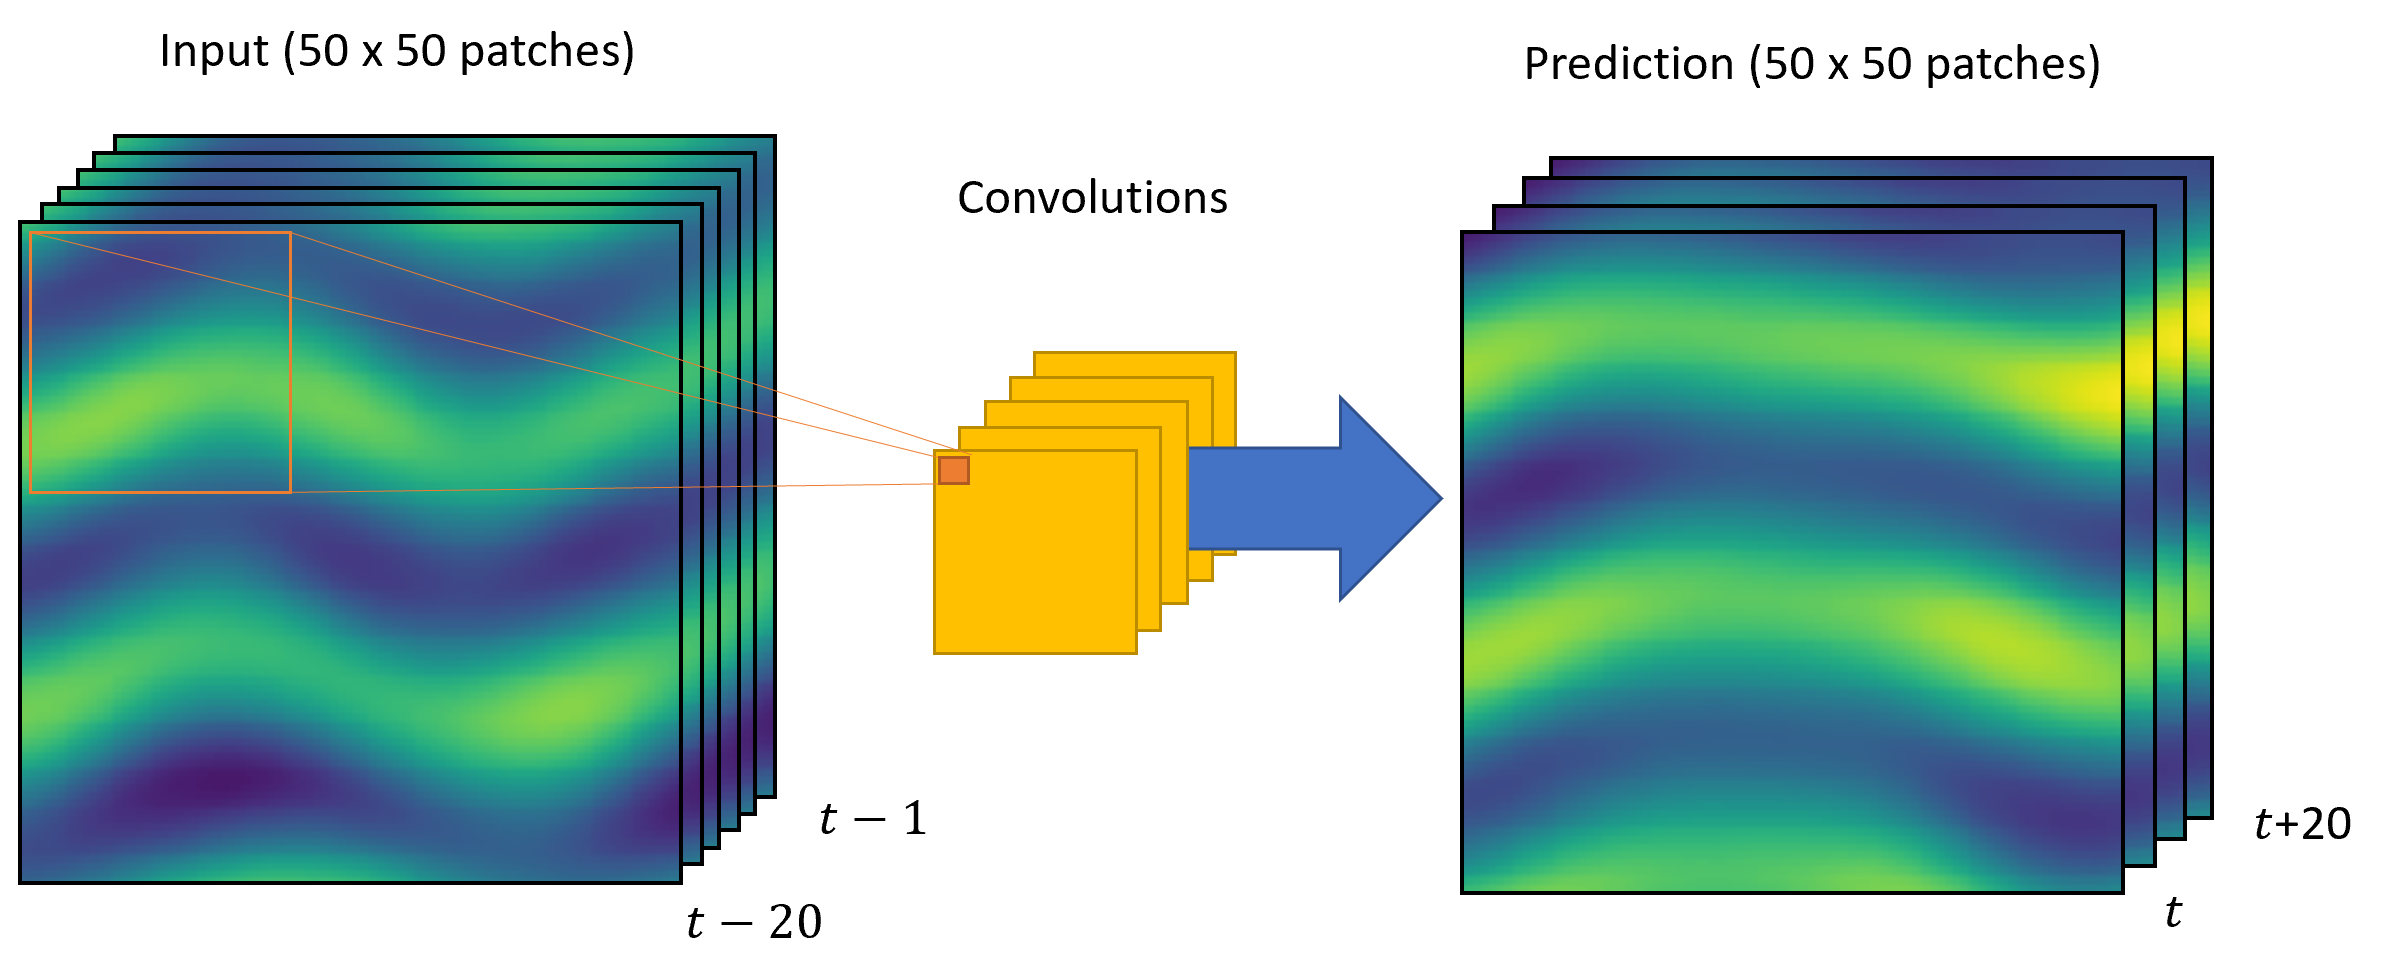
\includegraphics[width=0.7\textwidth]{images/network_conv.PNG}
		\caption{\small Demonstration of a simple convolutional network for predicting a time series. Depicted is a single convolutional layer followed by a fully connected output to map the convolutional features to the prediction. Twenty frames of history are given at a single 50px by 50px region $r$ of the turbulent flow and the network must predict the flow at the next 20 time-steps in the same region $r$.}
		\label{net_con}
	\end{center}	
\end{figure}

\begin{figure}
	\begin{center}
		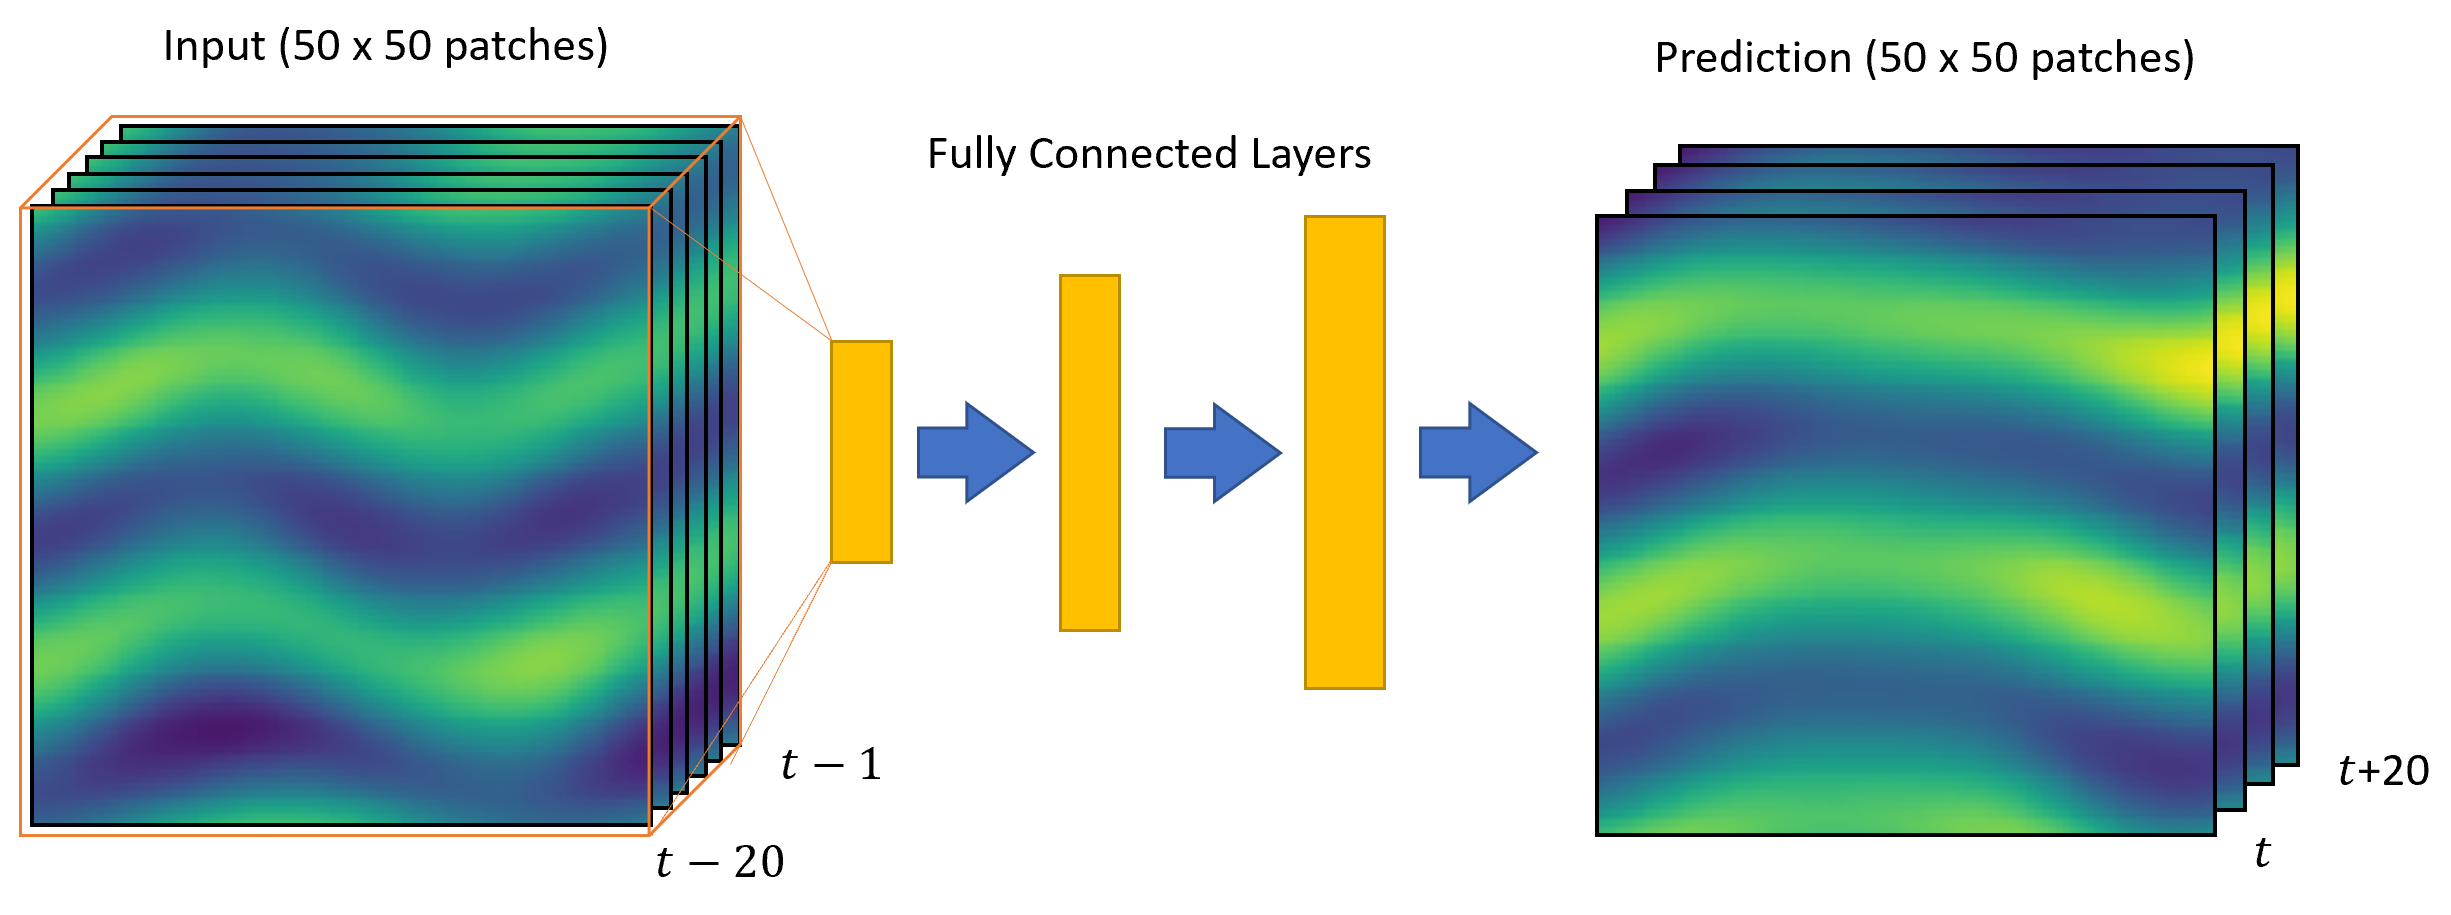
\includegraphics[width=0.7\textwidth]{images/network_fc.PNG}
		\caption{\small Demonstration of a three layer fully connected network. Three layers are use intermittently to determine the activation where each layer is densely connected to the one before it (a weight for each incoming edge.) Again twenty frames of history are given at a single 50px by 50px region $r$ of the turbulent flow and the network must predict the flow at the next 20 time-steps in the same region $r$.}
		\label{net_fc}
	\end{center}	
\end{figure}


In this period we expanded on our previous findings to attempt to predict a series of patches in a given region $r$ given 20 frames of history for that region $r$. Simply expanding the number of predicted frames for the previous network resulted in poor performance, where the network would converge to predicting the average for the data without learning to generalize well. To ensure the network had sufficient expressive power to represent the turbulent flow, we generated a set of low-dimensional periodic data by evaluating functions of $sin(x), cos(y)$. This allowed us to validate the learning procedure and correct some small bugs as well as verify that the proposed network architectures were able to interpret and generate 2D time series for periodic flow. Most convolutional networks tested showed artifacts during training, where as networks with fully connected layers before prediction were able to estimate the sinusoidal test data well.

\subsection{Formulation} \label{formulation}

\begin{figure}
	\begin{center}
		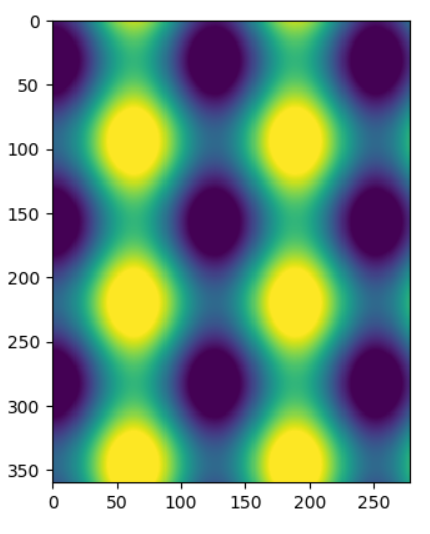
\includegraphics[width=0.35\textwidth]{images/sin_data_0.PNG}
		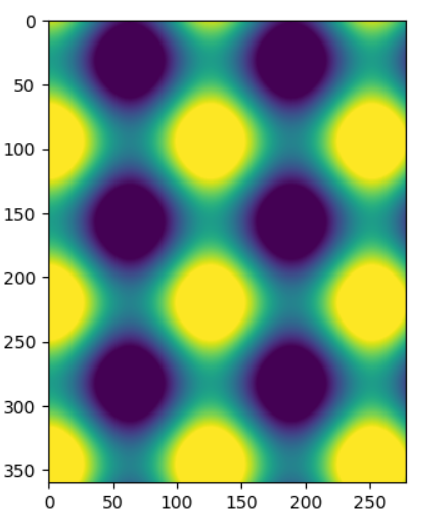
\includegraphics[width=0.35\textwidth]{images/sin_data_1.PNG}
		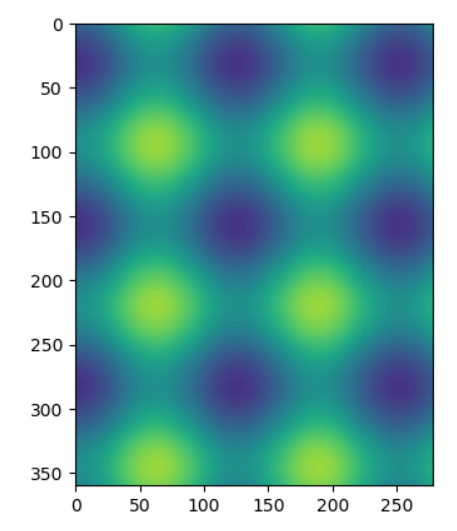
\includegraphics[width=0.35\textwidth]{images/sin_data_2.PNG}
		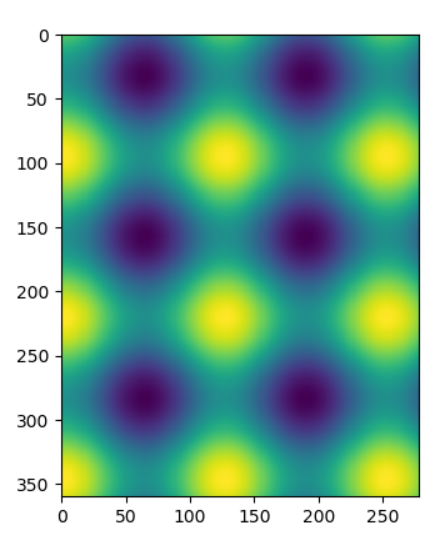
\includegraphics[width=0.35\textwidth]{images/sin_data_3.PNG}
		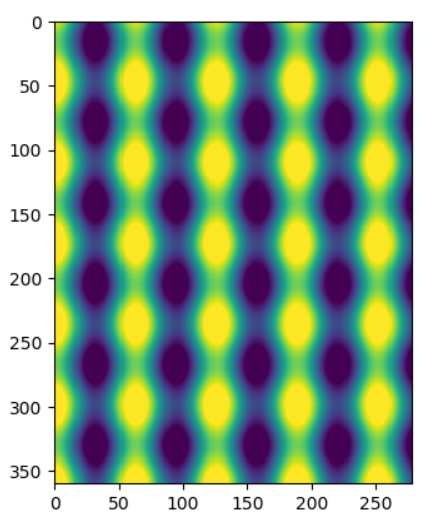
\includegraphics[width=0.35\textwidth]{images/sin_data_4.PNG}
		\caption{\small Single time step for five different functions of u,v,t where u,v represent the pixel co-ordinates from the top left and t represents the current frame. Starting at the top, left to right the functions respectively are: 
			1: $sin(u) * sin(t) + cos(v) * cos(t)$
			2: $sin(u) * sin(t) + cos(v) * cos(t/2)$
			3: $(sin(u) + cos(v)) * cos(t)$
			4: $sin(u + t) + cos(v + t / 2)$
			5: $sin(u*2) * sin(t*8) + cos(v*2) * cos(t*4)$}	
		\label{training}
	\end{center}	
\end{figure}



Let $P_t \in \mathbb{R}^{360*279} $ be the turbulent flow at time $t \in \{1, 2, ..., 1000\}$ and define a window $w_{(r, t)}$ of $P_t$ in terms of a 50px by 50px region $r \in \{(u,v) \mid u \in \{0, ..., 309\}, v \in \{0, ...,  228\}\}$ 
For a particular region and time $(r,t) \in (\mathbb{R}^2,\mathbb{R})$ the input $x$ is a series of windows in the past, given by:
 $$x = \{w_{(r,i)} \mid t-20 \leq i \leq t-1 \} \in \mathbb{R}^{50*50*20}$$ and our target $y$ is a single window of the form: $$y = \{w_{(r,i)} \mid i = t  \} \in \mathbb{R}^{50*50}$$

To train the network we randomly sample 5000 region, time pairs $S_i = \{(r, t) \mid i \in \{0, 1, ..., 4999\} \}$ and withhold 500 for validation creating two datasets, $X_{val} = \{w_{(S_i)} \mid i < 500 \} $ and $X_{train} = \{ {w_{(S_i)}\mid i \geq 500} \}$. We then learn a convolutional network $f(x)$ to minimize the huber loss, $L(y, f(x))$ given by:
$$L(y, f(x)) = \begin{cases}
	\max(0, 1 - y \, f(x))^2 & \textrm{for }\, \,  y \, f(x) \ge -1, \\
	-4y \, f(x)              & \textrm{otherwise.}
\end{cases}$$

The network $f(x)$ is composed of a series of convolutional or fully connected layers. Convolutional layers use 2D filters across all channels and are moved across the patch along the u,v axis. Fully connected layers use a matrix of weights maping each activation from the input to an activation of the hidden unit using a unique multiplicative weight for each. Training is conducted over \num{5e+8} batches of 128 input - label pairs using the TensorFlow back-end and Adam optimizer.


\subsection{Results}
 The network is able to achieve an average loss $L(y, f(x)) \leq 0.001$ and as shown in figure \ref{training}, the predicted turbulent flow matches the true distribution closely. Additionally, by observing the mean absolute difference, $\overline{Y_{(s_i)} - f(X_{(s_i)})}$ as shown in figure \ref{mean_error}, we see that the predictive error is relatively uniform and not concentrated along the edges of the window. This demonstrates that 

\subsubsection{Predicting Vorticity Dynamics}
The first formulation uses 20 frames of history to predict 20 future states as illustrated in figure \ref{net_con}. This existing network performed poorly, learning effectively the average over different patches, future work will use the new architectures and learning procedure updated durring the sinusoidal testing that we performed below.

\begin{figure}
	\begin{center}
		
\includegraphics[width=0.79\textwidth]{images/avg_perf_lab.png}
		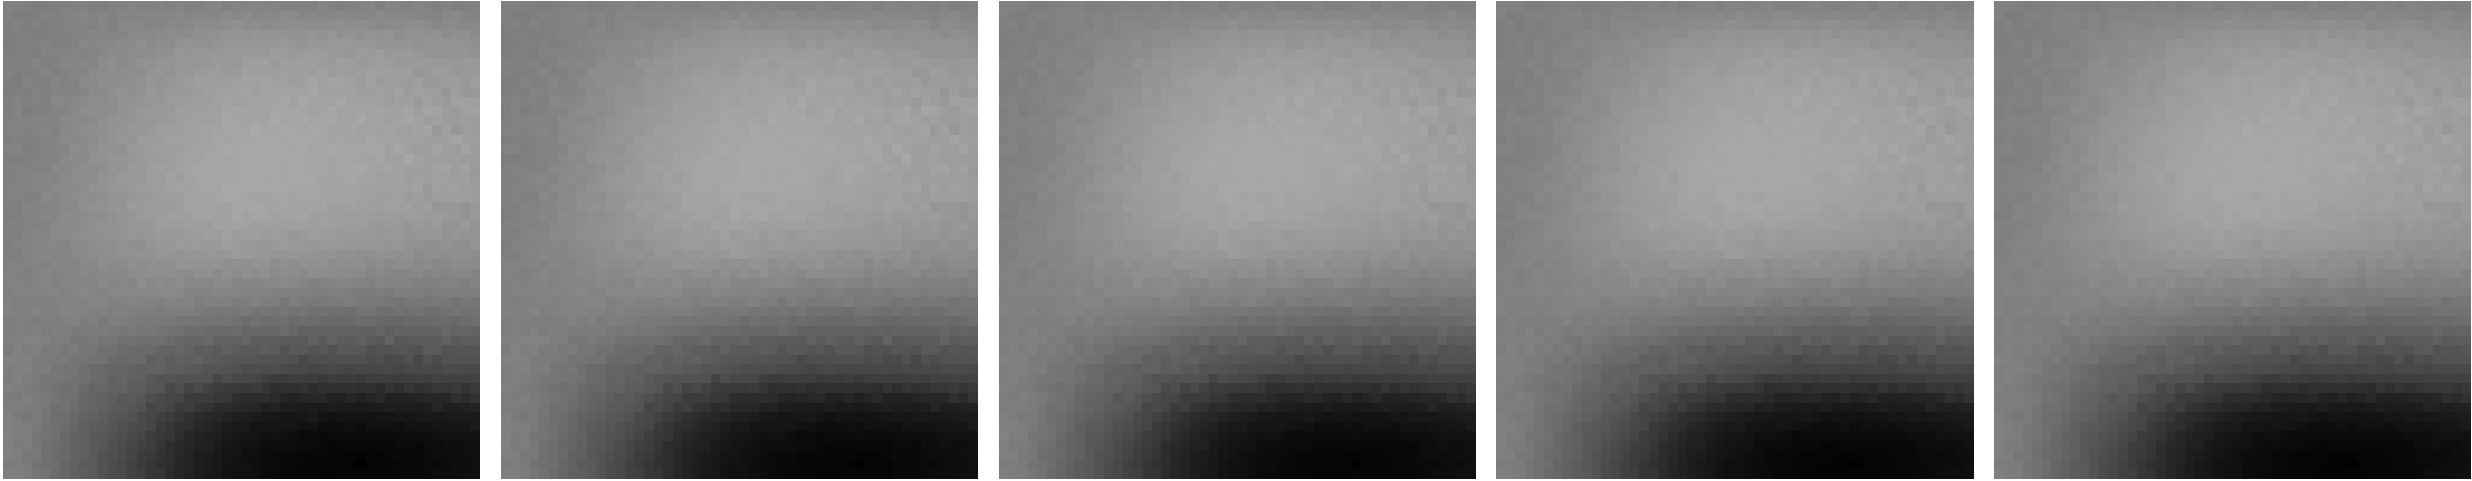
\includegraphics[width=0.79\textwidth]{images/avg_perf.png}
		\caption{\small Top: Label for prediction at t+5 steps. Bottom: Estimated value by network. Note the estimate for similar patches is the average over many patches and does not match any patch exactly. This effect is prevalent over images predicted both close (t) and far (t+19).}
		\label{mean_error}
	\end{center}	
\end{figure}

\subsubsection{Learning Low Dimensional Periodic Functions From Parameters}
To validate that the networks tested were learning properly we generated sinusoidal series as a function of pixel co-ordinates $u,v$ and time $t$. This allows us to predict the sinusoidal time series from the embedding as the embedding for the function is know. Thus we learn a deep network $f(u,v,t)$ to predict $sin^*(u,v,t) : \mathbb{R}^3 \longrightarrow \mathbb{R}^{50*50*20}$ where $sin^*$ represents a function composed of trigonometric functions evaluated for 20 time steps over a 50x50 patch in the range $0 \leq u \leq 360, 0 \leq v \leq 279$, e.g. $sin^* = sin(u) * sin(t) + cos(v) * cos(t)$. This network was able to predict the sinusoidal function from the parameters demonstrating its suitability for expressing such functions.


\subsubsection{Predicting Low Dimensional Periodic Function Dynamics}
Following the success of the function approximation above, we then learn the future value of the function from 20 previous frames of history, learning directly a function $f(P_t) = \hat{y}$ where $P_t$ is a patch taken from the sinusoidal function. We trained this network and it learns well, as shown in figure \ref{sin_perf}. This result was taken before the network converged (given the number of parameters in the network, takes a while to train). When the network is unrolled to predict time steps individually, we expect performance to improve dramatically.

\begin{figure}
	\begin{center}
		
\includegraphics[width=0.35\textwidth]{images/sin_0.PNG}
		
\includegraphics[width=0.35\textwidth]{images/sin_lab_0.PNG}
		
\includegraphics[width=0.35\textwidth]{images/sin_5.PNG}
		
\includegraphics[width=0.35\textwidth]{images/sin_lab_5.PNG}
		
\includegraphics[width=0.35\textwidth]{images/sin_10.PNG}
		
\includegraphics[width=0.35\textwidth]{images/sin_lab_10.PNG}	
		
\includegraphics[width=0.35\textwidth]{images/sin_15.PNG} 
		
\includegraphics[width=0.35\textwidth]{images/sin_lab_15.PNG}
		\caption{\small Left: learned sinusoidal function. Right: ground truth function value. Each row corresponds to a section in time, columns correspond to the 5 validation examples. Note that for some regions the network predicts well, but for others the predictions lose high frequency information and are more abstract than the true function. This is expected given the network did not finished training when these samples were taken.}	
		\label{sin_perf}
	\end{center}	
\end{figure}


\section{Future Work}
Using architectures that are able to accurately predict sinusoidal data, we aim to roll out those network using recurrent layers enabling the prediction of a sequence of turbulent flow from a fixed length of history. We will use this to generate an encoding of the history and use a decoder network to predict arbitrarily far into the future. We also hope to add random permutation to the data 


\end{document}